

\tikzset{every picture/.style={line width=0.75pt}} %set default line width to 0.75pt        

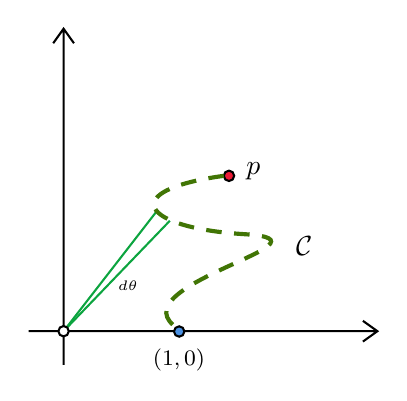
\begin{tikzpicture}[x=0.75pt,y=0.75pt,yscale=-1,xscale=1]
%uncomment if require: \path (0,204); %set diagram left start at 0, and has height of 204

%Straight Lines [id:da6296287507736172] 
\draw [color={rgb, 255:red, 12; green, 164; blue, 63 }  ,draw opacity=1 ]   (215.48,167.32) -- (260.68,109.1) ;
%Straight Lines [id:da5728376102170853] 
\draw [color={rgb, 255:red, 12; green, 164; blue, 63 }  ,draw opacity=1 ]   (215.48,167.32) -- (266.68,114.1) ;
%Shape: Axis 2D [id:dp2457846957791402] 
\draw  (198.68,167.32) -- (366.68,167.32)(215.48,21.58) -- (215.48,183.52) (359.68,162.32) -- (366.68,167.32) -- (359.68,172.32) (210.48,28.58) -- (215.48,21.58) -- (220.48,28.58)  ;
%Shape: Circle [id:dp471059490475613] 
\draw  [fill={rgb, 255:red, 255; green, 255; blue, 255 }  ,fill opacity=1 ] (212.98,167.32) .. controls (212.98,165.94) and (214.1,164.82) .. (215.48,164.82) .. controls (216.86,164.82) and (217.98,165.94) .. (217.98,167.32) .. controls (217.98,168.7) and (216.86,169.82) .. (215.48,169.82) .. controls (214.1,169.82) and (212.98,168.7) .. (212.98,167.32) -- cycle ;
%Shape: Circle [id:dp6796959702440949] 
\draw  [fill={rgb, 255:red, 236; green, 27; blue, 54 }  ,fill opacity=1 ] (292.67,92.46) .. controls (292.67,91.08) and (293.79,89.96) .. (295.17,89.96) .. controls (296.55,89.96) and (297.67,91.08) .. (297.67,92.46) .. controls (297.67,93.85) and (296.55,94.96) .. (295.17,94.96) .. controls (293.79,94.96) and (292.67,93.85) .. (292.67,92.46) -- cycle ;
%Shape: Circle [id:dp9329257413194855] 
\draw  [fill={rgb, 255:red, 74; green, 144; blue, 226 }  ,fill opacity=1 ] (268.67,167.46) .. controls (268.67,166.08) and (269.79,164.96) .. (271.17,164.96) .. controls (272.55,164.96) and (273.67,166.08) .. (273.67,167.46) .. controls (273.67,168.85) and (272.55,169.96) .. (271.17,169.96) .. controls (269.79,169.96) and (268.67,168.85) .. (268.67,167.46) -- cycle ;
%Curve Lines [id:da9676248064011552] 
\draw [color={rgb, 255:red, 65; green, 117; blue, 5 }  ,draw opacity=1 ][line width=1.5]  [dash pattern={on 5.63pt off 4.5pt}]  (292.67,92.46) .. controls (240.68,99.58) and (252.68,117.58) .. (302.68,120.58) .. controls (352.68,123.58) and (237.68,145.58) .. (271.17,166.46) ;

% Text Node
\draw (257,174.4) node [anchor=north west][inner sep=0.75pt]  [font=\footnotesize]  {$( 1,0)$};
% Text Node
\draw (326,120.4) node [anchor=north west][inner sep=0.75pt]    {$\mathcal{C}$};
% Text Node
\draw (240.08,141.61) node [anchor=north west][inner sep=0.75pt]  [font=\tiny]  {$d\theta $};
% Text Node
\draw (302,84.4) node [anchor=north west][inner sep=0.75pt]    {$p$};


\end{tikzpicture}
